\documentclass{article}
\usepackage[utf8]{inputenc}
\usepackage{geometry}
 \geometry{
 a4paper,
 total={170mm,257mm},
 left=20mm,
 top=20mm,
 }
 \usepackage{graphicx}
 \usepackage{titling}
 \usepackage{listings}
 \usepackage{enumerate}
 \usepackage{subcaption}
 \usepackage{float}
 \title{Parallelization of K-means clustering algorithm through MPI+OpenMP and CUDA
}
\author{Riccardo Inverardi Galli}
\date{January 2025}

 
 \usepackage{fancyhdr}
\fancypagestyle{plain}{%  the preset of fancyhdr 
    \fancyhf{} % clear all header and footer fields
    %\fancyfoot[R]{\includegraphics[width=2cm]{KULEUVEN_GENT_RGB_LOGO.png}}
    \fancyfoot[L]{\thedate}
    \fancyhead[L]{K-means project report}
    \fancyhead[R]{\theauthor}
}
\makeatletter
\def\@maketitle{%
  \newpage
  \null
  \vskip 1em%
  \begin{center}%
  \let \footnote \thanks
    {\LARGE \@title \par}%
    \vskip 1em%
    %{\large \@date}%
  \end{center}%
  \par
  \vskip 1em}
\makeatother

\usepackage{lipsum}  
\usepackage{fouriernc} % Added for Fourier New Century font

\begin{document}

\maketitle

\noindent\begin{tabular}{@{}ll}
    Student & \theauthor\\
     Course &  Programmazione di sistemi Embedded e Multicore\\
     Professor & Daniele de Sensi
\end{tabular}

\section*{Overview of K-means}
K-means is a machine learning clustering algorithm used to perform a classification task on a collection of points of arbitrary dimensionality. In k-means, the user chooses a number K of classes and the algorithm, given a set of points $P$ of cardinality $|P|=m$, where each point $p\in P$ has dimensionality $D$, such  that $$p_i=(p_{i_{1}}, p_{i_{2}},\ldots,p_{i_{D}}),\space 0\leq i<m$$ and given a set $C$ of centroids of cardinality $|C|=k$, each centroid of dimensionality $D$, will assign, over a series of iterations, each point to a centroid $c\in C$. The assignment of a point is performed by computing the euclidean distance $$\sqrt{(p_i - c_j)^2}$$ between a point $i$ and each centroid $j$ and choosing the smallest between these values. This procedure is summarized in the following formula, which also takes into account the dimensionality $D$ of points 
\begin{equation}
    \min_{0\leq k <K}\sqrt{\sum_{d=1}^{D}(x_{i_d}-c_{k_d})^2}
    \label{eq:mindist}
\end{equation}
where $x_{i_d}$ is the d-th component of point $i$. The sequential version of the program provides the following straightforward implementation of euclidean distances:
\begin{lstlisting}
    float euclideanDistance(float *point, float *center, int samples)
{
	int i;
	float dist=0.0;
	for(i = 0; i < samples; i++)
	{
		dist+= (point[i]-center[i])*(point[i]-center[i]);
	}
	dist = sqrt(dist);
	return(dist);
}
\end{lstlisting}
It is important to point out that centroids do not possess any special properties. Initially, they are just points chosen at random from the set of points $P$, and after the first iteration each centroid $c_k$ is computed as the average of all points $p$ that are assigned to $k$. 
\begin{equation}
    c_k=\frac{1}{|K_i|}\sum_{i\in K_i}x_i
    \label{eq:newcentroid}
\end{equation}
%$$c_k=\frac{1}{|K_i|}\sum_{i\in K_i}x_i$$ 
\\The K-means algorithm works as follows:
\begin{enumerate}
    \item Select K random centroids from the point cloud $P$.
    \item Assign each point $p \in P$ to the nearest centroid by picking the smallest Euclidean distance for that point from all the distances between that point and all centroids (using ~\ref{eq:mindist}).
    \item Recalculate the centroids of each cluster as the mean of the data points assigned to each cluster (using ~\ref{eq:newcentroid}).
    \item Repeat steps 2 and 3 until:
    \begin{enumerate}
        \item The centroids do not change significantly; i.e. between one iteration and the previous one, the maximum movement of all centroids within each cluster is less than a given threshold.
        \item The number of data point that move from one cluster to another between one iteration and the previous one is less than a given threshold.
        \item A predefined maximum number of iterations is reached.
    \end{enumerate}
\end{enumerate}
\section*{MPI+OpenMP}
The first implementation leverages the parallelization opportunities presented by using in conjunction MPI and OpenMP. MPI is a standard designed to function on parallel computing architectures, based on the SPMD (single program, multiple data) paradigm, where multiple autonomous processors simultaneously execute the same program at independent points, while OpenMP is a API that supports multi-platform shared memory multi-processing programming. \\The approach chosen when combining these two parallel programming paradigms  was very simple: Because of the nature of K-means, the only factors that can significantly increase the runtime of the application are
\begin{enumerate}
    \item Cardinality $|P|$ of the point cloud.
    \item Dimensionality of the points
\end{enumerate}
The most straight-forward approach was to split the data cloud between a fixed number of MPI processes, and then parallelize the rest of the computation using OpenMP pragmas. This approach works very well due to the nature of the K-means algorithm; Since the heaviest computation at each iteration is computing the Euclidean distance of all points from each centroid (with $m$ points and $K$ centroids, we must perform $mK$ distance calculations), scattering the points through $n$ MPI processes reduces the theoretical computation time by a factor $n$ (there are no dependencies between computing distances of two points $i$ and $j$, $i\neq j$). This works because there is no redundant computation between processes, and each process $i$ computes it's own part of $$[p_l, p_{l+1}, \ldots, p_j]_{1\leq l \leq j \leq m} \circ([c_{1},\ldots,c_{k}])$$
where $p_l\in P$, $c_j \in C$, and $\circ$ denotes the application of the Euclidean distance algorithm for each $p$.\\ To further increase parallelization OpenMP is used to parallelize for loops. This setup requires some calculations on the number of threads OpenMP can use. We want to have 
\begin{lstlisting}
    MPI_proc + OMP_threads = CPU_cores
\end{lstlisting}
This number tends to be different on each system, thus we set the number of OpenMP threads to 
\begin{lstlisting}
    int nthreads=NLOGIC_CORES / comm_sz;
    omp_set_num_threads(nthreads);
\end{lstlisting}
where \textbf{NLOGIC\_CORES} is the total number of logic cores of the system and is a compile time constant, and \textbf{comm\_sz} is a runtime variable containing the size of MPI's communicator (the number of processes we specify with the -n flag of mpirun). This setup ensures that we are always using the full capacity of the CPU. To know the value of \textbf{NLOGIC\_CORES}, we can run the following command on UNIX systems:
\begin{lstlisting}
    lscpu | grep -E "^Thread|^Core|^Socket|^CPU\("
\end{lstlisting}
By default, MPI creates a copy of all buffers for each process (SPMD), thus we only need to allocate two additional arrays, one to store the local part of the point cloud in each process, and another to store the local class map for the local point could (although during each iteration we allocate two additional utility arrays). A class map is an array the indicates to what centroid $k$ a point $i$ belongs. \\The program contains three parallel sections that do most of the computation for one iteration, while the last loop is performed sequentially for each MPI process, since the number of operations is too small to justify further parallelization overhead.\\ To distribute the point cloud between MPI processes, we first allocate this buffer:
\begin{lstlisting}
    int local_sz = lines / comm_sz;

    /* Thread local bufffers */
    float local_data[local_sz*samples];
    int* local_classMap = (int*)calloc(local_sz,sizeof(int));
\end{lstlisting}
Here, \textbf{lines} contains $|P|$ (number of points), and \textbf{samples} is an integer indicating the dimensionality $D$ of each point. To store a fraction of the point cloud, we initialize \textbf{local\_data} as a one dimensional array, and we address different points using row-major order. This kind of ordering allows us to abstract 2D arrays while still storing points contiguously in memory. To access dimension $j$ of point $i$, we translate $A[i][j]$ in $A[i*D + j]$. After the allocation we use MPI\_Scatter to distribute the point cloud evenly, choosing process 0 as the root process for simplicity, although any other process could have done it.
\begin{lstlisting}

    /* Scatter data array */
    if (rank == 0)
    {
        MPI_Scatter(data, local_sz*samples, MPI_FLOAT, local_data, 
        local_sz*samples, MPI_FLOAT, root, COMM);
    } else
    {
	MPI_Scatter(NULL, local_sz*samples, MPI_FLOAT, local_data, 
        local_sz*samples, MPI_FLOAT, root, COMM);
    }
\end{lstlisting}
Initially, there are very few differences between the sequential version and this implementation. The flexibility of OpenMP pragmas allows to leave the code virtually untouched, excluding the limits of the loop and the arrays to work on, which are now bound to each local instance of the data cloud. The variables \textbf{changes} and \textbf{local\_classMap} are declared as shared in the pragma, while the rest of the variables are kept private to each spawned thread. It is necessary to increment \textbf{changes} atomically to avoid race conditions and to ensure that the final value is the correct one. This is crucial because \textbf{changes} is a variable that determines a possible exit condition, so we must be very careful when dealing with it to make sure that we don't accidentally lose some data.
\begin{lstlisting}
    it++;
    changes = 0;
    #pragma omp parallel for shared(local_classMap, changes)\
    private(i, _class, minDist, k, dist)
    for (i = 0; i < local_sz; i++) /* Iterate over each point */
    {
	_class = 1;
	minDist = FLT_MAX;
        for (k = 0; k < K; k++) /* Iterate over each centroid */
	{
            dist=euclideanDistance(&local_data[i*samples], &centroids[k*samples], samples);

	   if(dist < minDist)
	   {
		minDist=dist;
		_class=k+1;
	   }
        }
        if(local_classMap[i] != _class)
        {
            #pragma omp atomic
	    changes++;
        }
        local_classMap[i]=_class;
    }
\end{lstlisting}
The second part of the program needed some modifications from the original sequential version. In the sequential program computing the new centroids is done in two steps:
\begin{enumerate}
    \item Accumulate all the values of points belonging to each class.
    \item Divide the accumulate values by the number of points belonging to each class.
\end{enumerate}
This approach must be changed in the parallel version because at this point of the algorithm processes do not share a common view of the data cloud. Each process can only accumulate to each class the number of points it was assigned. To solve this problem, we allocate two arrays to store a local version of \textbf{auxCentroids} and \textbf{pointsPerClass}. We use these arrays to handle local computation and then use a critical section to update the global (to each MPI process) arrays. After we are done with this step, we call MPI\_Allreduce on \textbf{pointsPerClass}, \textbf{auxCentroids}, and \textbf{changes}, so that now all MPI processes share a common view of the accumulated values. Note that the last accumulation step (summing up all the values from all the different processes) is performed by the Allreduce operation. \\After Allreduce is called, all the processes share a common view of the accumulated values and the number of points belonging to each class, and it's possible to perform the last step of centroid calculation, which is dividing by the number of points that belong to each class $k$. We use the special \textbf{MPI\_IN\_PLACE} flag to tell MPI that we wish to perform the Allreduce operation using the same array as sending and receiving array.
\begin{lstlisting}
    #pragma omp parallel
    {
        int* local_pointsPerClass = (int*) calloc(K, sizeof(int));
        float* local_auxCentroids = (float*) calloc(K*samples, sizeof(float));

        #pragma omp for private(_class, i, j)
        for (int i = 0; i < local_sz; i++)
        {
            _class = local_classMap[i];
            local_pointsPerClass[_class-1] += 1;
            for(int j = 0; j < samples; j++)
            {
                local_auxCentroids[(_class-1)*samples+j] += local_data[i*samples+j];
            }
        }
        #pragma omp critical
        {
            for (int k = 0; k < K; k++)
            {
                pointsPerClass[k] += local_pointsPerClass[k];
                for (int j = 0; j < samples; j++)
                {
                    auxCentroids[k * samples + j] += local_auxCentroids[k * samples + j];
                }
            }
        }
        free(local_pointsPerClass);
        free(local_auxCentroids);
    }
    MPI_Allreduce(MPI_IN_PLACE, pointsPerClass, K, MPI_FLOAT, MPI_SUM, COMM);
    MPI_Allreduce(MPI_IN_PLACE, auxCentroids, K*samples, MPI_FLOAT, MPI_SUM, COMM);
    MPI_Allreduce(MPI_IN_PLACE, &changes, 1, MPI_INT, MPI_SUM, COMM);
    #pragma omp parallel for shared(pointsPerClass, auxCentroids) private(k, j)
    for(k = 0; k < K; k++)
    {
        for(j = 0; j < samples; j++)
        {
            auxCentroids[k*samples+j] /= pointsPerClass[k];
        }
    }
\end{lstlisting}
After this step is performed, the computation for one iteration is finished. The new centroids have been computed, and all that is left is to compute the distance between the old centroids stored in \textbf{centroids} and the new ones stored in \textbf{auxCentroids}. This has to be done in order to check if the new centroids are at a significant distance from the old ones. If they are not, the algorithm is free to terminate. This last part is left sequential for each MPI process, and is identical to the original sequential code. 
\begin{lstlisting}
    maxDist=FLT_MIN;
    for(k = 0; k < K; k++)
    {
        distCentroids[k] = euclideanDistance(&centroids[k*samples], &auxCentroids[k*samples], samples);
        if(distCentroids[k]>maxDist)
        {
            maxDist=distCentroids[k];
        }
    }
    memcpy(centroids, auxCentroids, (K*samples*sizeof(float)));
\end{lstlisting}
\section*{CUDA}
CUDA is Nvidia's proprietary parallel computing API which allows programmers to access a Nvidia GPU instruction set through the C++ programming language. GPU architectures are specifically made to leverage parallelism and high bandwidth communication inside each device, through a very high number of cores and several levels of in-device memory.\\
To parallelize the K-means clustering algorithm on a GPU, since the main factor that influences runtime of the application is the number of points the algorithm has to iterate on, it was natural to think that the algorithm should be parallelized over each point. By assigning to each core in every streaming multiprocessor (SM) a point in the point cloud it is possible to speed up the application considerably.\\ 
Constants that are used frequently by kernels are placed in constant memory so that they can be quickly broadcasted to all cores on the device. In particular, we declare three variables that are very frequently used as constant variables, and during the memory allocation phase they are set to their values with cudaMemcpyToSymbol.
\begin{lstlisting}
    __constant__ int samples_d;
    __constant__ int K_d;
    __constant__ int lines_d;
    ...
    CHECK_CUDA_CALL( cudaMemcpyToSymbol(samples_d, &samples, sizeof(int)) );
    CHECK_CUDA_CALL( cudaMemcpyToSymbol(K_d, &K, sizeof(int)) );
    CHECK_CUDA_CALL( cudaMemcpyToSymbol(lines_d, &lines, sizeof(int)) );
\end{lstlisting}
Similarly to what we did with MPI+OpenMP version, we still have to compute the euclidean distance of all points from all centroids at every iteration of the algorithm. To avoid high latency issues that come from communicating with global memory, because each core computing values for a single point would have to request from global memory every centroid, we place in shared memory of every SM the entire array containing the centroids. In order to do this, we must address two problems:
\begin{enumerate}
    \item We do not know a priori the size of the centroids array, since both the dimensionality and the number of centroids are known only at runtime
    \item We have a limited amount of shared memory in each SM
\end{enumerate}
On Nvidia devices with a 7.5 compute capability like the ones that are available on sapienza's cluster, there is a unified data cache of 96Kb, and a part of it can be reserved to be allocated as shared memory (32Kb or 64Kb). The programmer must specify the percentage of total shared memory capability he wants to use for each kernel that needs shared memory usage. To do this, we must use cudaFuncSetAttribute(), passing to it as arguments the kernel, what attribute we wish to set (in our case shared memory carveout), and the percentage of shared memory we wish to allocate.
\begin{lstlisting}
    int carveout = 100;
    ...
    CHECK_CUDA_CALL( cudaFuncSetAttribute(firstStepGPU,
    cudaFuncAttributePreferredSharedMemoryCarveout, carveout) );
\end{lstlisting}
Since the centroids array can be arbitrarily big, and the dimensionality of points can go up to 100 in our test cases, we set the carveout to 100, thus reserving the whole 64K shared memory space, in order to be sure that we can fit at most 16384 4 byte floating point numbers in it (which should be enough for any centroids array). It is important to note that this must be done only for those kernels that require shared memory. \\ 
Another issue with shared memory is dynamic allocation, since we are not able to statically allocate shared memory in a kernel like so:
\begin{lstlisting}
    __shared__ float sharedCentroids[K_d*samples_d];
\end{lstlisting}
This allocation would result in a compilation error unless \textbf{K\_d} and \textbf{samples\_d} are compile time constants, which they are not. To fix this problem, we must dinamically allocate shared memory by declaring an unspecified size array, using the \textbf{extern} keyword, and then passing the size of the array as a parameter of the kernel call:
\begin{lstlisting}
    KERNEL CODE
    extern __shared__ float sharedCentroids[];
    ...
    DEVICE CODE
    firstStepGPU<<<dimGrid, dimBlock, csize>>>(...kernel arguments...);
\end{lstlisting}
Computing the euclidean distance is done through a \textbf{\_\_device\_\_} version of the provided \textbf{euclideanDistance} function, called \textbf{euclideanDistanceGPU}. The implementation is virtually identical, with the exception that the dimensionality of the points must not be passed as an argument to the function because it's a broadcasted constant from constant memory.
\begin{lstlisting}

   
__device__
float euclideanDistanceGPU(float* point1 /* in  */,   /* Point 1 */
                           float* point2 /* in  */)   /* Point 2 */
{
	float dist = 0.0;
	for (int i = 0; i < samples_d; i++)
	{
		dist += (point1[i] - point2[i]) * (point1[i] - point2[i]);
	}
	dist = sqrtf(dist);
	return (dist);
}
\end{lstlisting}
After all the logic for parallelization is set up, the individual code each thread executes is very similar to the sequential version. The blocks are organized as a one dimensional of size 64, and the block grid is also one dimensional of size 72. The code calls four kernels:
\begin{enumerate}
    \item \textbf{fistStepGPU}: It computes the distance of each point from all the centroids, and saves in classMap[p] the closest centroid to point p.
    \item \textbf{recalculateCentroidsStep1GPU}: It computes the values needed for the calculation fo the new centroids. After the execution, auxCentroids will have stored the (not normalized) sum of all points that belong to each class, and pointsPerClass will contain the count of all points belonging to each class.
    \item \textbf{recalculateCentroidsStep2GPU}: It divides the sum of the values of all the points belonging to class k by the number of points belonging to class k.
    \item \textbf{recalculateCentroidsStep3GPU}: Checks whether the distance between the old centroids and the new ones is below the given threshold
\end{enumerate}
Communication with the device is done through two \textbf{cudaMemcpy} function calls at the end of the computation for each iteration, copying the number of changes and the maximum movement of the new centroids.\\
Although this CUDA implementation works well, more work could be done on it to greatly improve speed. One approach could be to reduce the number of kernels in order to minimize overhead, think of more efficient ways to allocate shared memory, and try to leverage the GPU ability to run concurrent kernels, although the latter would require to completely revisit the logic of the program, that at the current moment has dependecy issues between the kernels. 
\section*{Performance}
Performance was evaluated using several metrics. With the implementation that uses MPI in conjunction with OpenMP it was necessary to establish what combination of MPI processes and OpenMP threads was best over different input files. The tests where run on a 64 logical cores CPU, and multiple runs where performed on all configurations to capture the average runtime. For some metrics, like strong scaling and weak scaling, it was necessary to generate additional point clouds, not included in the test files. These point clouds where randomly generated by analyzing the biggest test file available (100k points of 100 dimensions), identifying the minimum and maximum value over all dimensions of all points, and picking from a uniform distribution in that range. The files generated have 200k, 400k,800k and 1.6M points, although it was not possible to use the biggest file in the MPI+OpenMP, possible due to MPI memory requirements. \\
Figure 1(a) shows average runtimes over the given test files with an increasing number of MPI processes. The remaining threads are created by OpenMP (i.e. for $n$ MPI processes, each process spawns $64/n$ OpenMP threads).
This plot shows that small files run more quickly when there is a small number (2-4) of MPI processes, and the rest of the parallelization is done through OpenMP. This suggest that below a certain size threshold most of the runtime is influenced by communication overhead between MPI processes, which tends to increase when we increase the number of processes, and OpenMP overhead.\\
This is further confirmed, although by different means, by Figure 1(b), which shows how for small files, while keeping the numbers of MPI processes fixed to two, and increasing the number of total threads created by the program through OpenMP, runtimes tend to slowly grow after a sharp decrease, indicating that the program does not display weak or strong scaling properties for small files.\\
For a dataset large enough (100D2, 100k points of $D=100$), we see in Figure 1(a) that runtime displays a parabolic behavior when increasing MPI parallelization, reaching a minimum at 8 MPI processes. This suggest that this particular setup is the most optimal for files large enough, and again confirms that communication overhead plays a crucial role in performance. Figure 1(d) shows strong scaling behavior when we give the program a large enough data set, with the number of MPI processes fixed to 8. Figure 1(e) shows similar behavior on larger datasets, but the speedup tends to decrease, suggesting that larger datasets might benefit from a different configuration.\\
CUDA version shows significant speedups only on very large cloud points, where it is faster than the parallel MPI+OpenMP version by a factor of 2 (1.6 vs 0.75 on average), and orders of magnitude faster than the sequential version (around 1.3 seconds of average vs 60 seconds on the largest dataset).
\section*{Conclusions}
This work shows the great opportunities presented by parallelizing programs that already work well sequentially.\\
If we wish to parallelize on a CPU, with minimum effort we can obtain tremendous speedups over large datasets, without needing to think of a different implementation of the problem. The combination of MPI and OpenMP showed great results over problems that do not have dependencies over the computation on the dataset. If it's possible to split the dataset and work independently on subsets of it, and if this approach does not increase the number of operations needed, we can have very good results, very quickly.\\
Although CPU parallelization works very well, using a GPU architecture can greatly boost performance, with the downside of greater complexity when writing programs, cost issues with respect to hardware, and harder debugging environments. Despite the challenges it poses, working with a GPU (or multiple GPUs) is by far the best method if one seeks performance and does not care much about cost, and should be an area of great interest for a programmer that is approaching parallel programming.

\begin{figure}[p]
    \centering
    \begin{subfigure}{0.40\textwidth}
        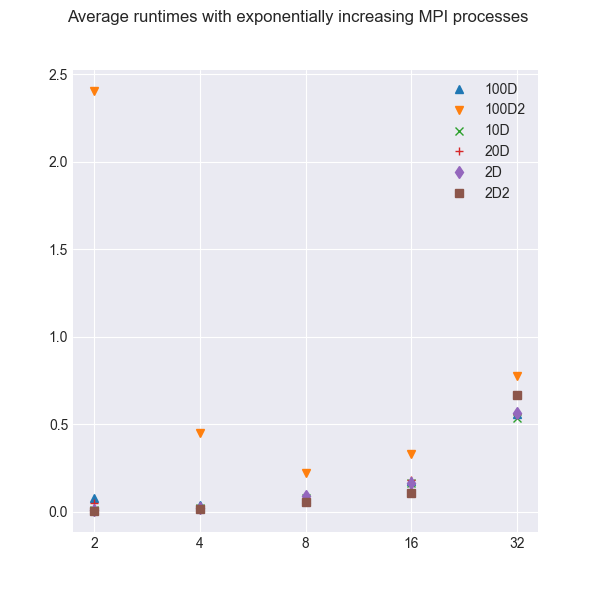
\includegraphics[width=\textwidth]{png/Average-runtimes.png}
        \caption{Average runtimes with different MPI configurations}
        \label{fig:image1}
    \end{subfigure}
    \begin{subfigure}{0.40\textwidth}
        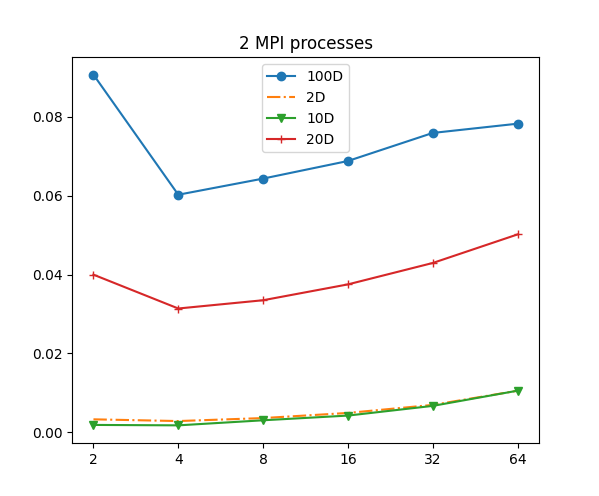
\includegraphics[width=\textwidth]{png/2MPIprocesses-smallTestFiles.png}
        \caption{Average runtimes with increasing OpenMP threads and two MPI processes}
        \label{fig:image2}
    \end{subfigure}
    \begin{subfigure}{0.40\textwidth}
        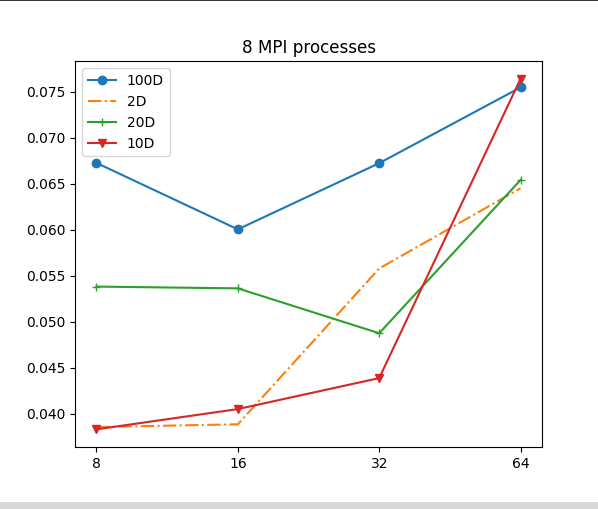
\includegraphics[width=\textwidth]{png/8MPIprocesses-smallTestFiles.png}
        \caption{Average runtimes with increasing OpenMP threads and eight MPI processes}
        \label{fig:image3}
    \end{subfigure}
    \begin{subfigure}{0.40\textwidth}
        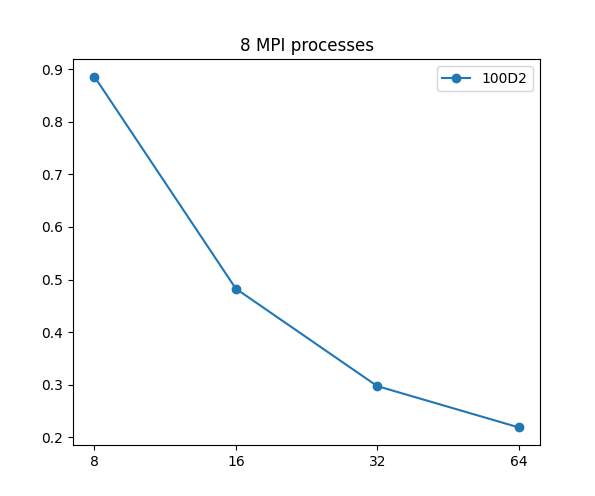
\includegraphics[width=\textwidth]{png/8MPIprocesses-bigTestFile.png}
        \caption{Average runtimes with increasing OpenMP threads and eight MPI processes}
        \label{fig:image4}
    \end{subfigure}
    \begin{subfigure}{0.40\textwidth}
        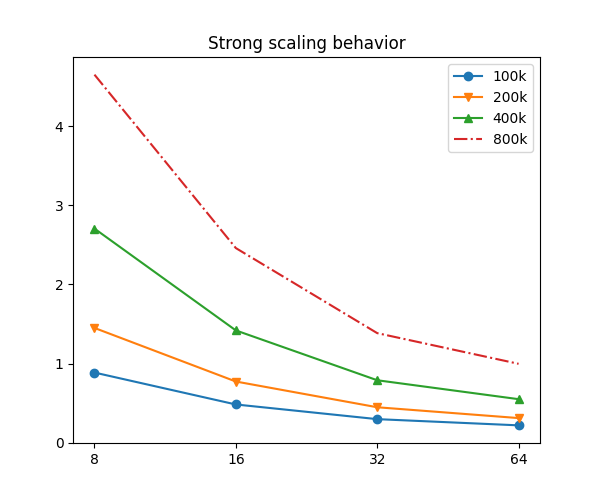
\includegraphics[width=\textwidth]{png/StrongScaling.png}
        \caption{Same as (d), bigger datasets}
        \label{fig:image5}
    \end{subfigure}
    \begin{subfigure}{0.40\textwidth}
        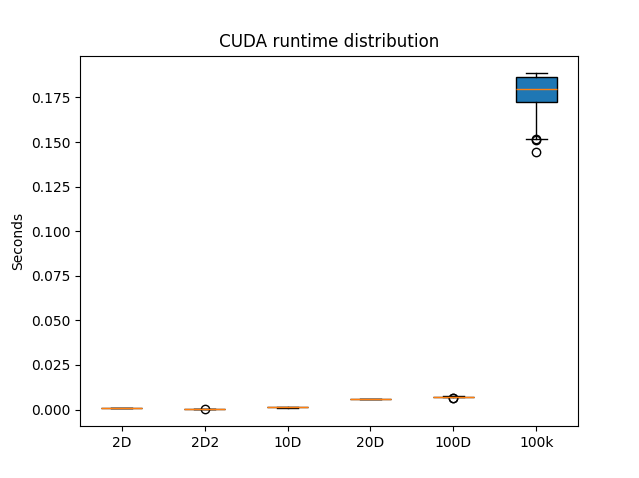
\includegraphics[width=\textwidth]{cudaRuntimeDistribution-1.png}
        \caption{CUDA runtimes on provided datasets}
        \label{fig:image6}
    \end{subfigure}
    \begin{subfigure}{0.40\textwidth}
        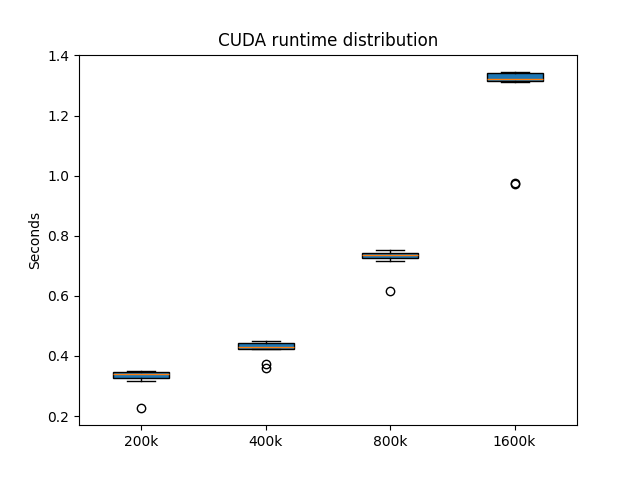
\includegraphics[width=\textwidth]{cudaRuntimeDistribution-2.png}
        \caption{CUDA runtimes on generated datasets}
        \label{fig:image7}
    \end{subfigure}
    %\caption{Overall caption for the images.}
    \label{fig:bothimages}
\end{figure}

\clearpage
\begin{figure}[H]
    \centering
     \begin{subfigure}{0.40\textwidth}
        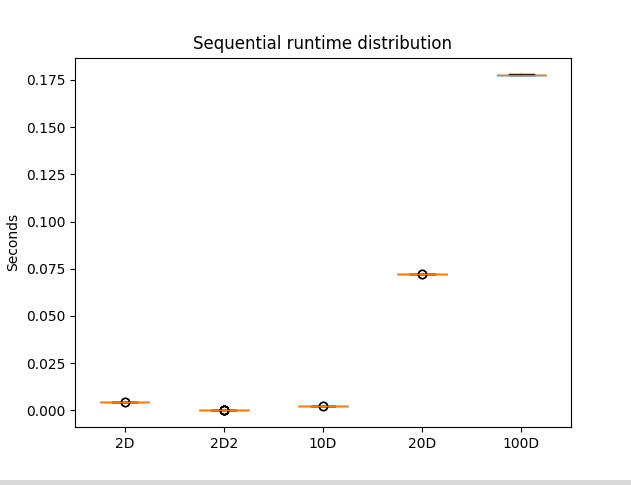
\includegraphics[width=\textwidth]{sequentialRuntimeDistribution-1.png}
        \caption{Sequential runtimes on provided datasets}
        \label{fig:image1}
    \end{subfigure}
     \begin{subfigure}{0.40\textwidth}
        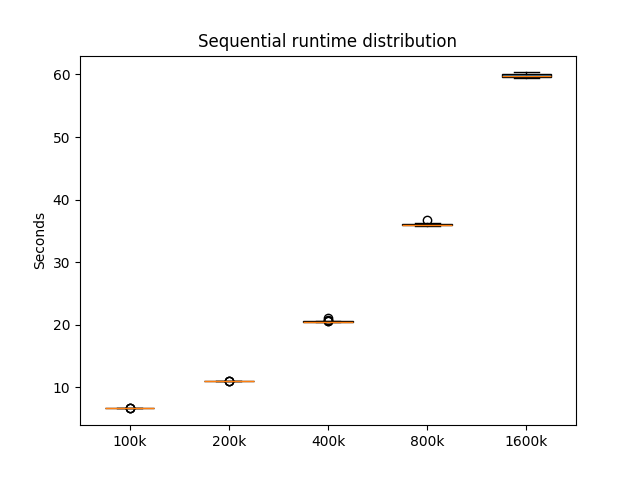
\includegraphics[width=\textwidth]{sequentialRuntimeDistribution-2.png}
        \caption{Sequential runtimes on generated datasets}
        \label{fig:image2}
    \end{subfigure}
\end{figure}
\end{document}
